\begin{appendix}
    \chapter{Annexes}
    
\newpage
\begin{figure}[H]
\begin{center}
\includegraphics[height=0.92\textheight, keepaspectratio]{images/show_online_cut.png}
\caption{Utilisation de la fonction d'affichage des variables avec mise à jour à chaque itérations.}
On compte une fenêtre par état/commande, excepté pour la fenêtre \emph{muscles\_actives}, qui regroupe trois états. Les itérations renvoyées par le solveur défilent dans le cadre jaune.
\label{fig:show_online_violon}
\end{center}
\end{figure} 



\newpage
    
    
\label{code_pendule_bioMod}
\begin{center}
\lstinputlisting{code/pendule.bioMod}
\vspace{-0.6cm}
\begin{figure}[ht]
\caption{Modèle pendule.bioMod.}
\end{figure}
\end{center}
\newpage

\label{code_pendule_python}
\begin{center}
\lstinputlisting[linewidth=18cm, xleftmargin=0cm]{code/pendule.py}
\vspace{-0.6cm}
\begin{figure}[h]
\caption{Programmation du problème du pendule.}
\end{figure}
\end{center}
\newpage

\begin{center}
\label{eocar}
\lstinputlisting[linewidth=18cm, xleftmargin=0cm]{code/eocar/eocar.py}
\vspace{-0.6cm}
\begin{figure}[h]
\caption{Définition du problème eocar.}
\end{figure}
\end{center}
\newpage

\begin{center}
\label{init}
\lstinputlisting[linewidth=18cm, xleftmargin=0cm]{code/biorbd_optim/__init__.py}
\vspace{-0.6cm}
\begin{figure}[h]
\caption{Fichier \emph{biorbd\_optim/\_\_init\_\_.py}}
\end{figure}
\end{center}

\begin{center}
\label{s2m1}
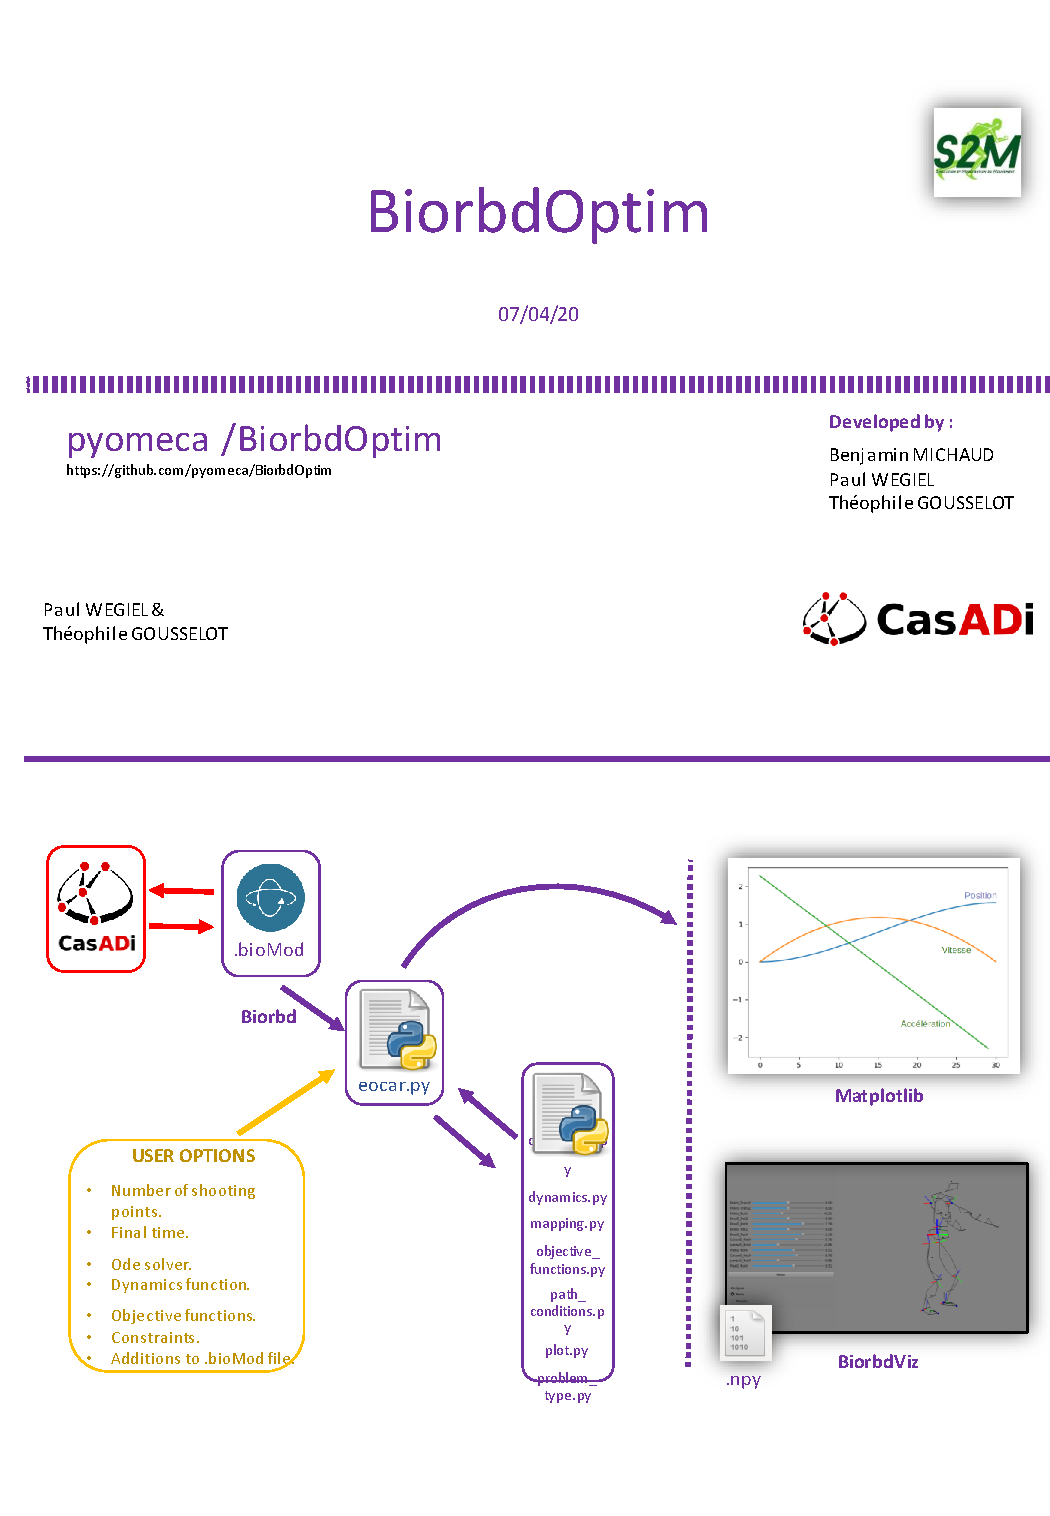
\includepdf[pages=-, width=17cm]{pdf/S2M1.pdf}
\vspace{-0.6cm}
\begin{figure}[h]
\caption{Première présentation à l'attention des membres de l'équipe de commande optimale.}
\end{figure}
\end{center}

\begin{center}
\label{s2m2}
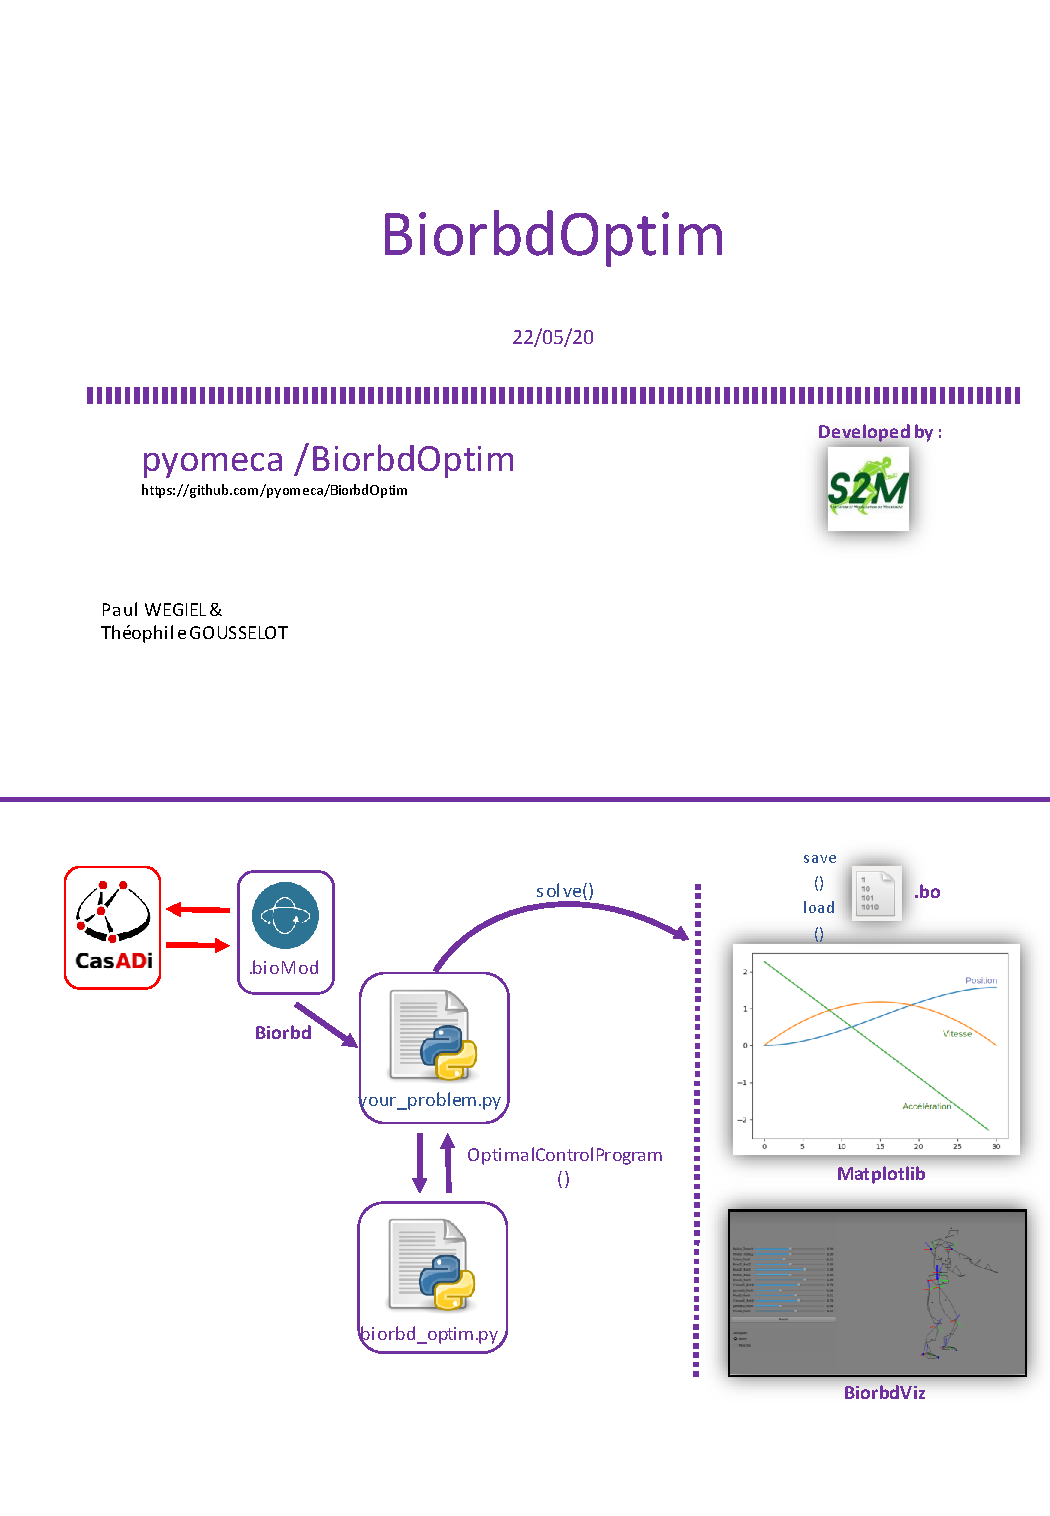
\includepdf[pages=-, width=17cm]{pdf/S2M2.pdf}
\vspace{-0.6cm}
\begin{figure}[h]
\caption{Deuxième présentation à l'attention des membres du laboratoire S2M.}
\end{figure}
\end{center}


\end{appendix}
